\subsubsection{Galvanic skin reaction and temperature data;}
\label{subsubsec:results_gsr_temp_2}

Table \ref{tab:gsr_table_noBase} presents the average skin conductance for both groups, while the percentual variation related to the baseline is presented in Table \ref{tab:gsr_var_blind}.


\begin{table}[!htb]
\centering
\caption{Average GSR felled by the participants [$\mu$S].}
\label{tab:gsr_table_noBase}
\begin{tabular}{lllrrrrrr}
\toprule
    &       &        & Baseline &  Audio & \begin{tabular}[c]{@{}l@{}}Haptic\\ Belt\end{tabular} & \begin{tabular}[c]{@{}l@{}}Virtual\\ Cane\end{tabular} & Mixture \\
Participant & Visual Condition & Round &          &        &                                                       &                                                        &         \\
\midrule
001C & Blind & First &     0.37 &   1.03 &                                                  3.14 &                                                   3.79 &    3.90 \\
    &       & Return &          &   1.58 &                                                  2.81 &                                                   4.04 &    4.57 \\
003C & Blind & First &     0.30 &   0.56 &                                                  0.62 &                                                   0.85 &    1.09 \\
    &       & Return &          &   0.63 &                                                  0.65 &                                                   0.92 &    1.06 \\
004C & Blind & First &     1.24 &   3.07 &                                                  3.49 &                                                   2.28 &    2.23 \\
    &       & Return &          &   2.95 &                                                  3.20 &                                                   2.21 &    2.24 \\
001 & Sight & First &     4.27 &  15.19 &                                                 15.67 &                                                  15.19 &   14.15 \\
    &       & Return &          &  14.95 &                                                 15.09 &                                                  15.72 &   21.52 \\
004 & Sight & First &     2.60 &  11.18 &                                                 12.60 &                                                  12.92 &   10.34 \\
    &       & Return &          &  11.97 &                                                 12.25 &                                                  13.47 &   10.16 \\
005 & Sight & First &     0.47 &   1.58 &                                                  1.44 &                                                   1.37 &    1.33 \\
    &       & Return &          &   1.53 &                                                  1.47 &                                                   1.49 &    1.33 \\
\bottomrule
\end{tabular}
\end{table}




\begin{table}[!htb]
\centering
\caption{Average GSR variation in relation to the baseline in each round [$\mu$S].}
\label{tab:gsr_var_noBase}
\begin{tabular}{lllrrrrrr}
\toprule
    &       &        &     Audio & \begin{tabular}[c]{@{}l@{}}Haptic\\ Belt\end{tabular} & \begin{tabular}[c]{@{}l@{}}Virtual\\ Cane\end{tabular} &    Mixture \\
Participant & Visual Condition & Round &           &                                                       &                                                        &            \\
\midrule
001 & Sight & First &  255.76\% &                                              266.93\% &                                               255.69\% &   231.52\% \\
    &       & Return &  250.18\% &                                              253.32\% &                                               268.25\% &   403.90\% \\
001C & Blind & First &  176.54\% &                                              746.10\% &                                               920.72\% &   951.71\% \\
    &       & Return &  327.42\% &                                              656.99\% &                                               988.93\% &  1132.39\% \\
003C & Blind & First &   84.23\% &                                              104.19\% &                                               182.35\% &   258.80\% \\
    &       & Return &  109.23\% &                                              112.95\% &                                               202.35\% &   249.72\% \\
004 & Sight & First &  329.08\% &                                              383.54\% &                                               395.83\% &   297.05\% \\
    &       & Return &  359.53\% &                                              370.35\% &                                               417.17\% &   289.96\% \\
004C & Blind & First &  148.53\% &                                              182.84\% &                                                84.33\% &    80.69\% \\
    &       & Return &  138.64\% &                                              159.00\% &                                                78.73\% &    81.61\% \\
005 & Sight & First &  239.16\% &                                              207.74\% &                                               193.85\% &   184.71\% \\
    &       & Return &  227.06\% &                                              214.91\% &                                               219.59\% &   185.86\% \\
\bottomrule
\end{tabular}
\end{table}



The barplots of the two groups are presented in Figure \ref{fig:barplot_gsr_avg_4_scene_blind_sight}. While the GSR varied for the blind participants, increasing for methods with vibration, the same does not happen for sighted participants. Also, the variance of GSR data for blind participants is significantly higher than that of sighted ones. The same conclusion can be drawn from the boxplots in Figures \ref{fig:boxplot_ecg_sdnn_4_scene} and \ref{fig:boxplot_ecg_sdnn_4_rounds}. 

\begin{figure}[!htb]
    \centering
    \begin{minipage}{\textwidth}
        \centering
        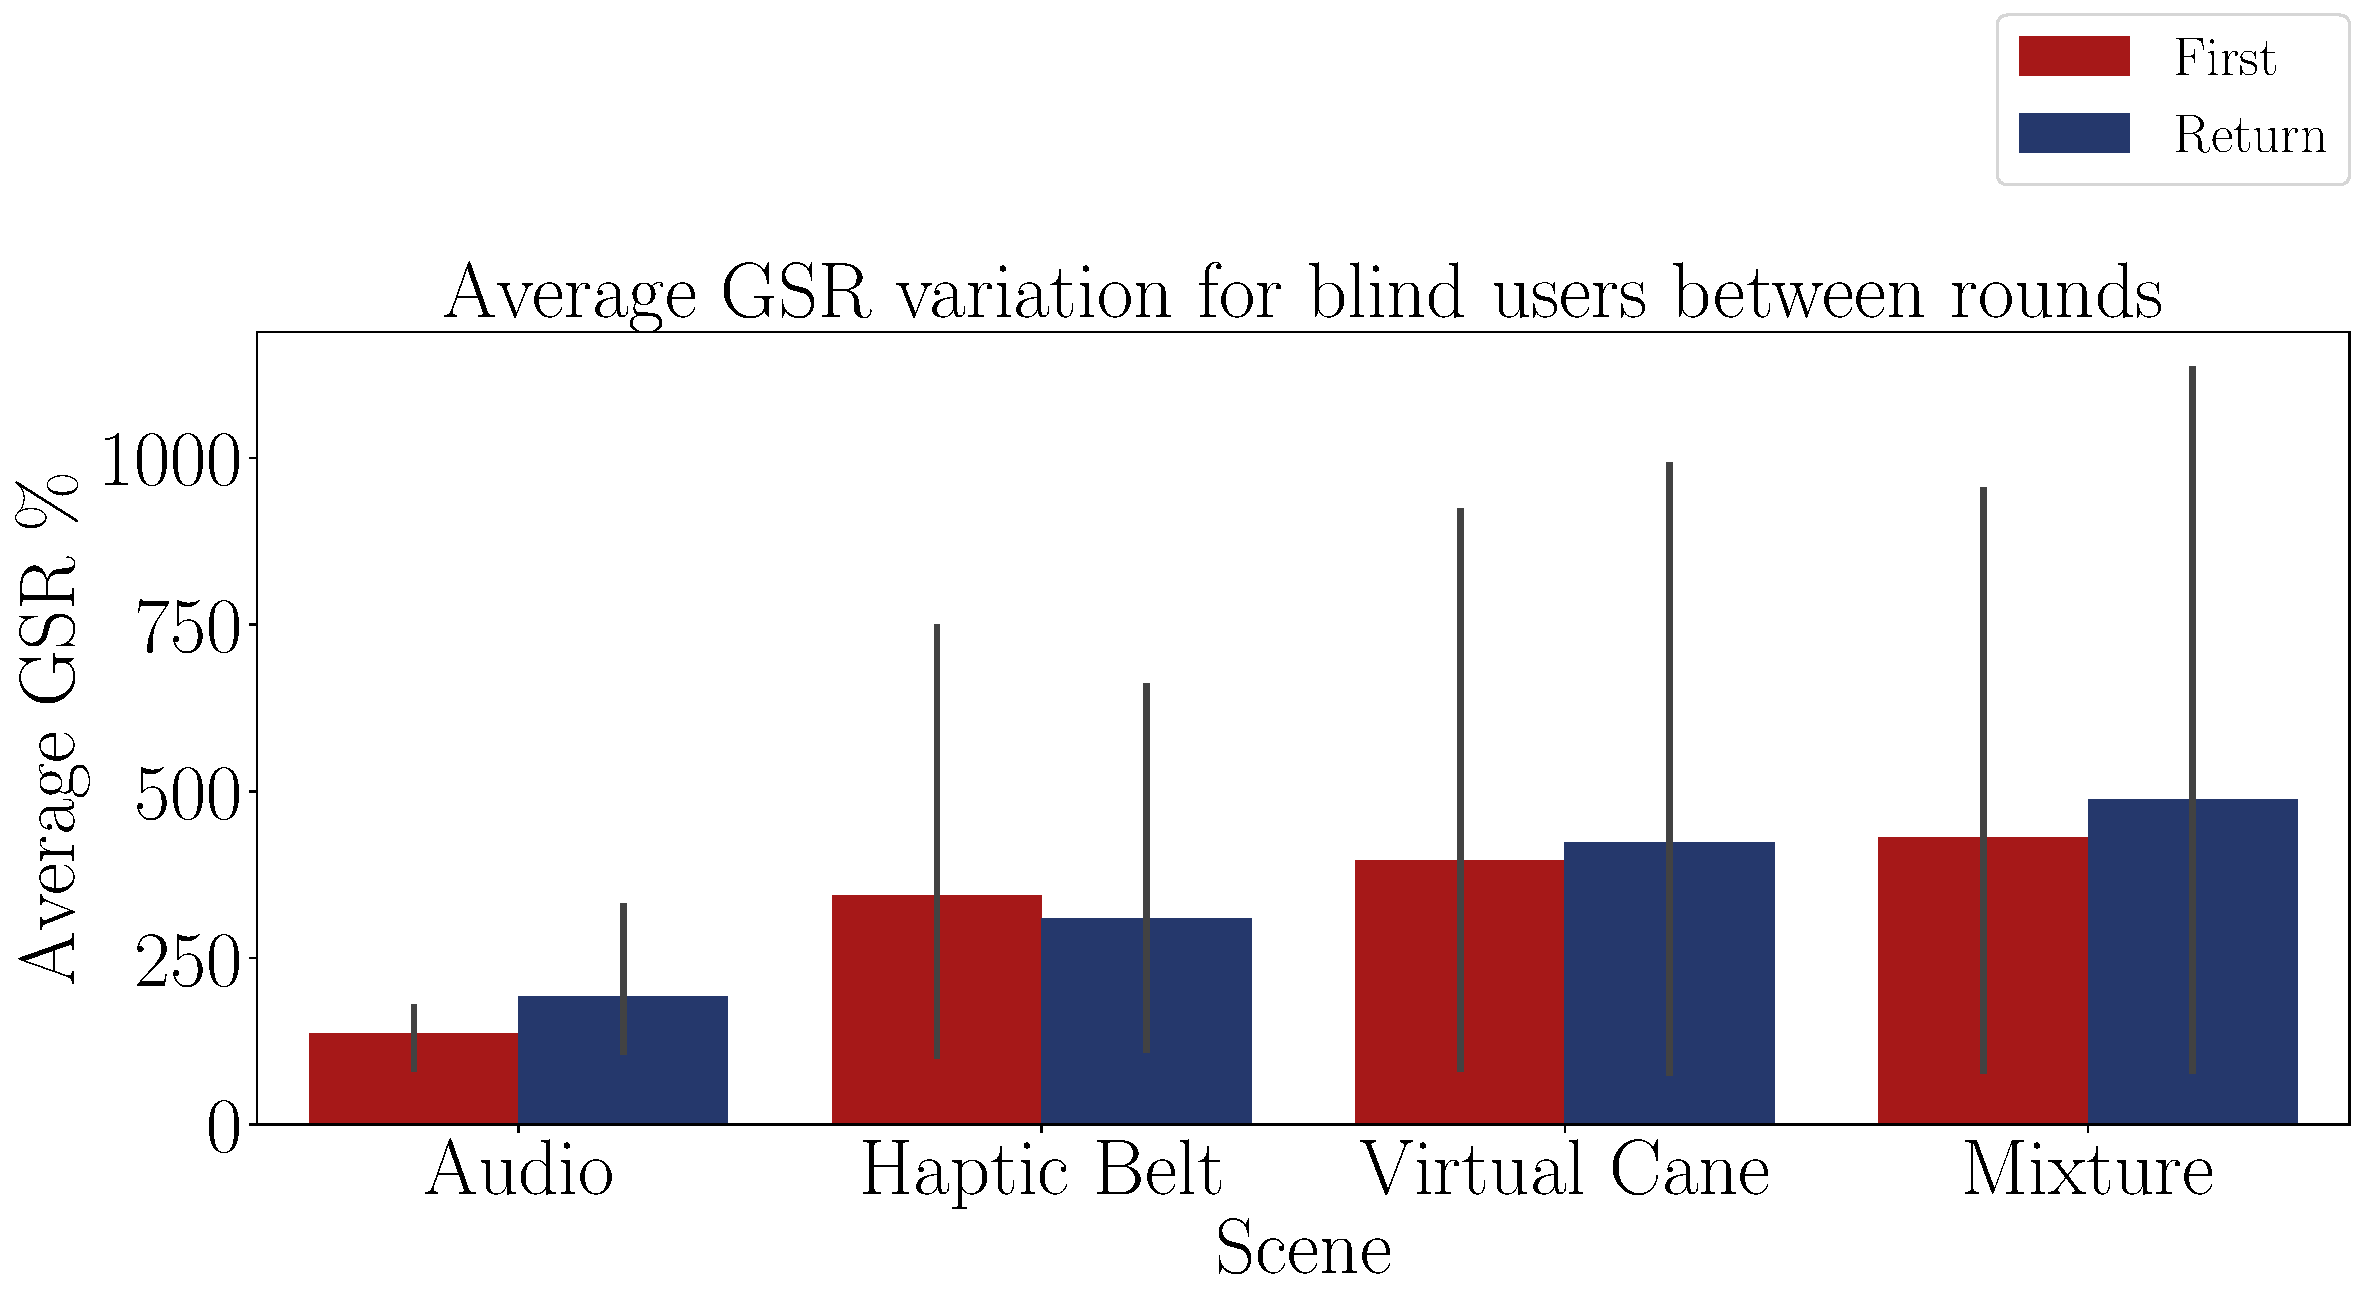
\includegraphics[width = \textwidth]{Resultados/GSR/Figuras/pdf/barplot_gsr_avg_4_scene_blind.pdf}
        \subcaption{Blind participants.}
        \label{fig:barplot_gsr_avg_4_scene_blind}
    \end{minipage}
    \begin{minipage}{\textwidth}
        \centering
        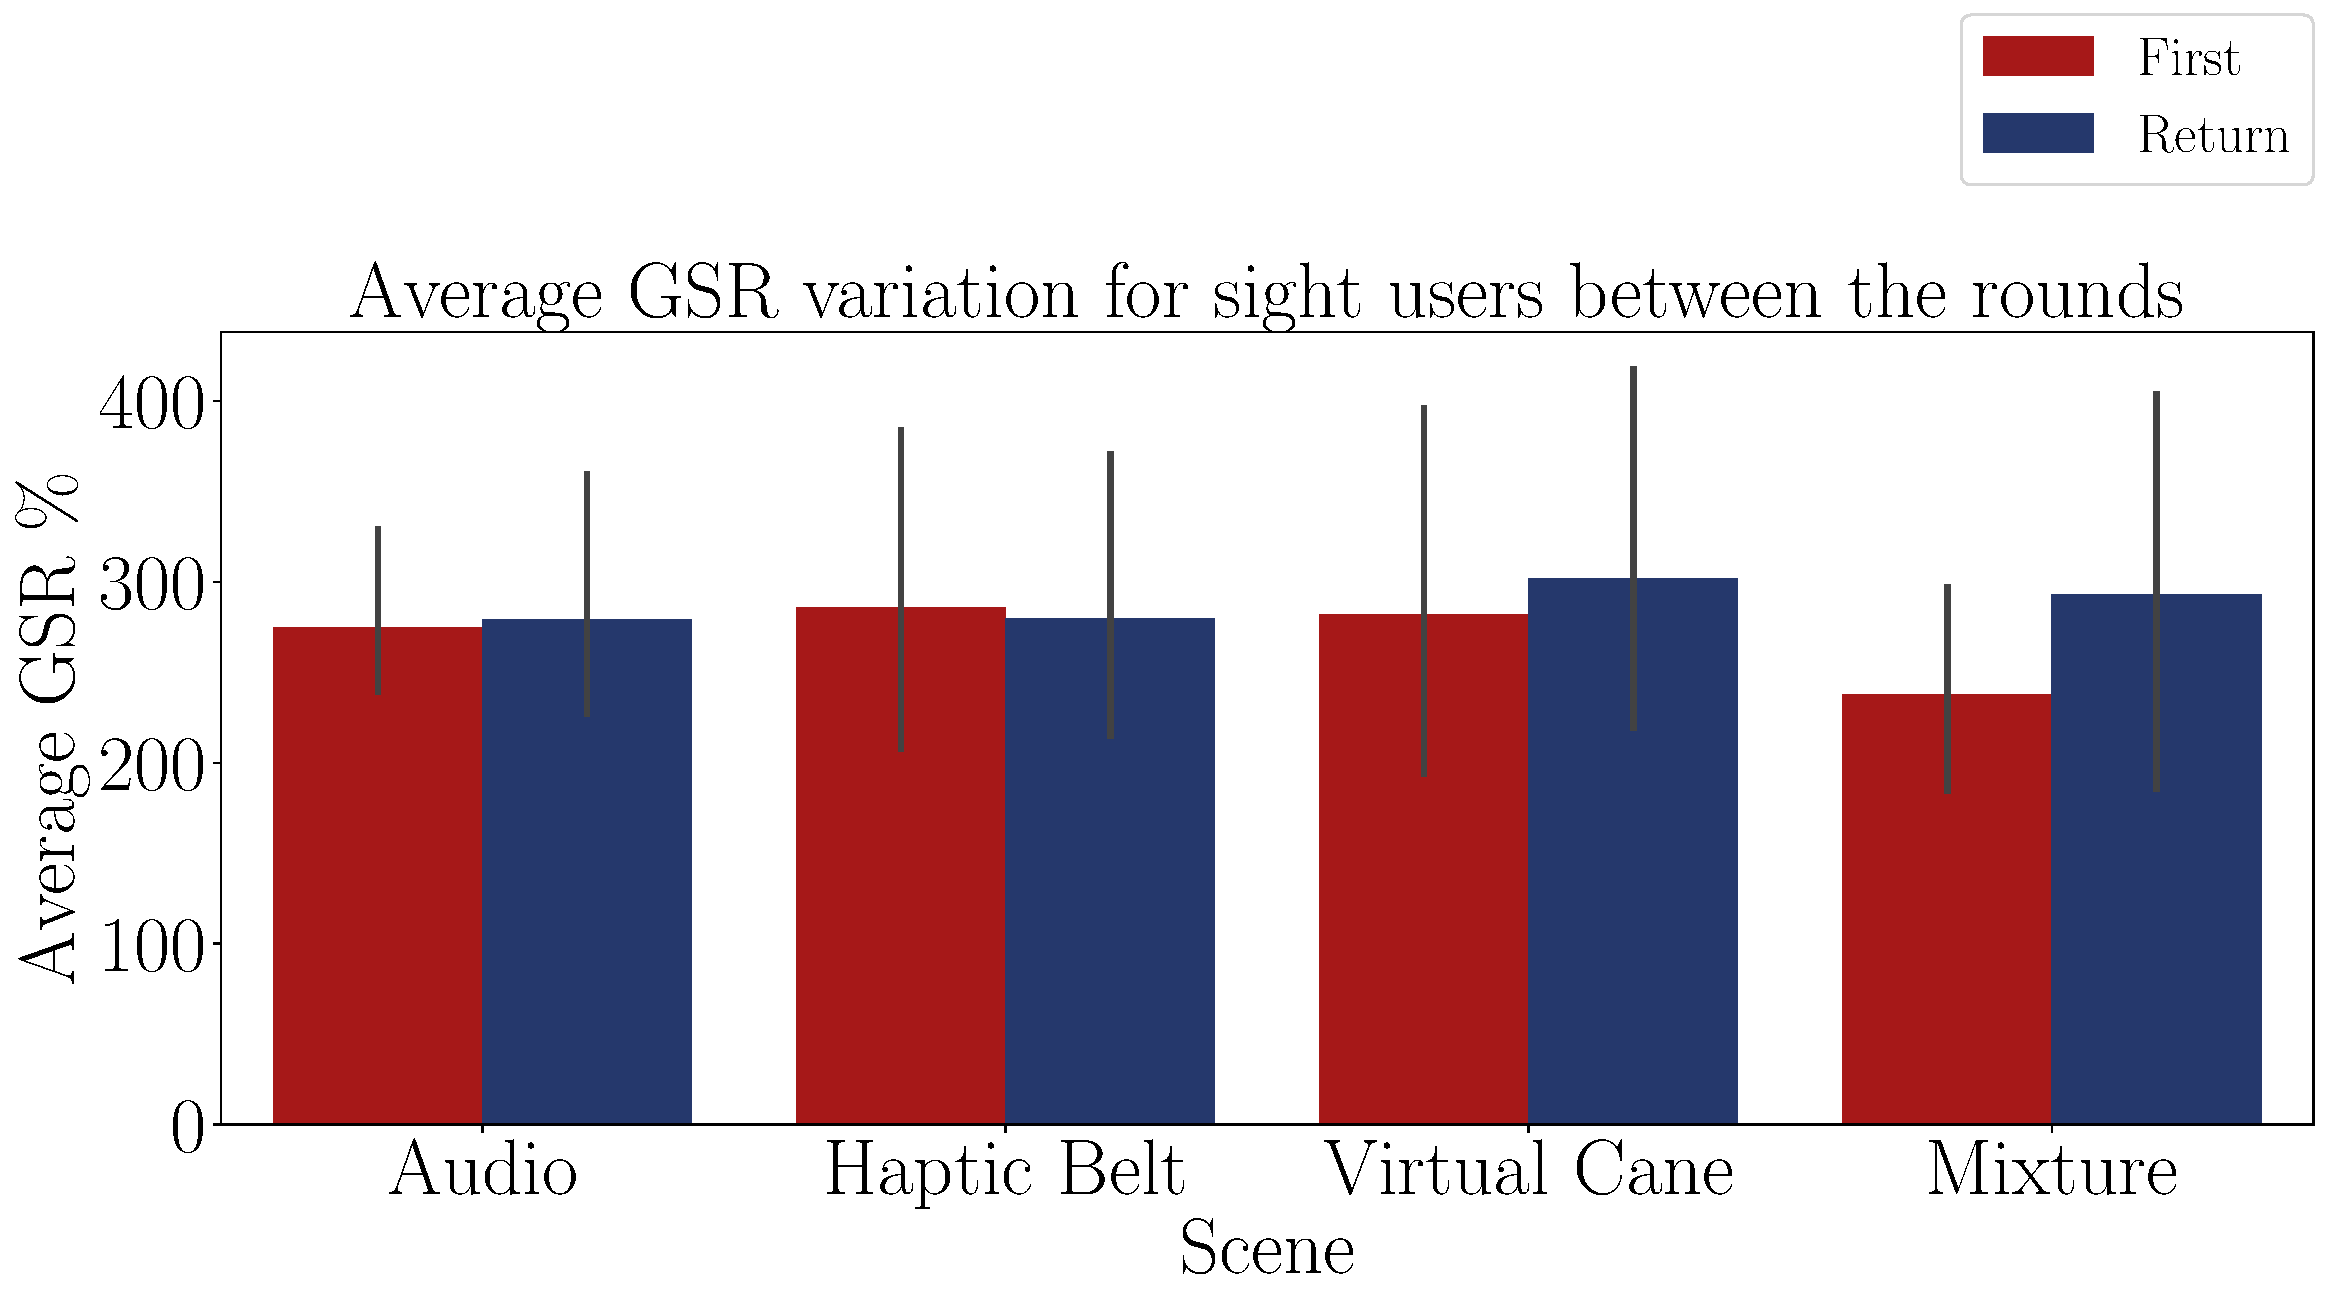
\includegraphics[width = \textwidth]{Resultados/GSR/Figuras/pdf/barplot_gsr_avg_4_scene_sight.pdf}
        \subcaption{Sight participants.}
        \label{fig:barplot_gsr_avg_4_scene_sight}
    \end{minipage}
    \caption{Barplot of the average GSR on each method and round.}
    \label{fig:barplot_gsr_avg_4_scene_blind_sight}
\end{figure}

\begin{figure}[!htb]
    \centering
    \begin{minipage}{0.45\textwidth}
        \centering
        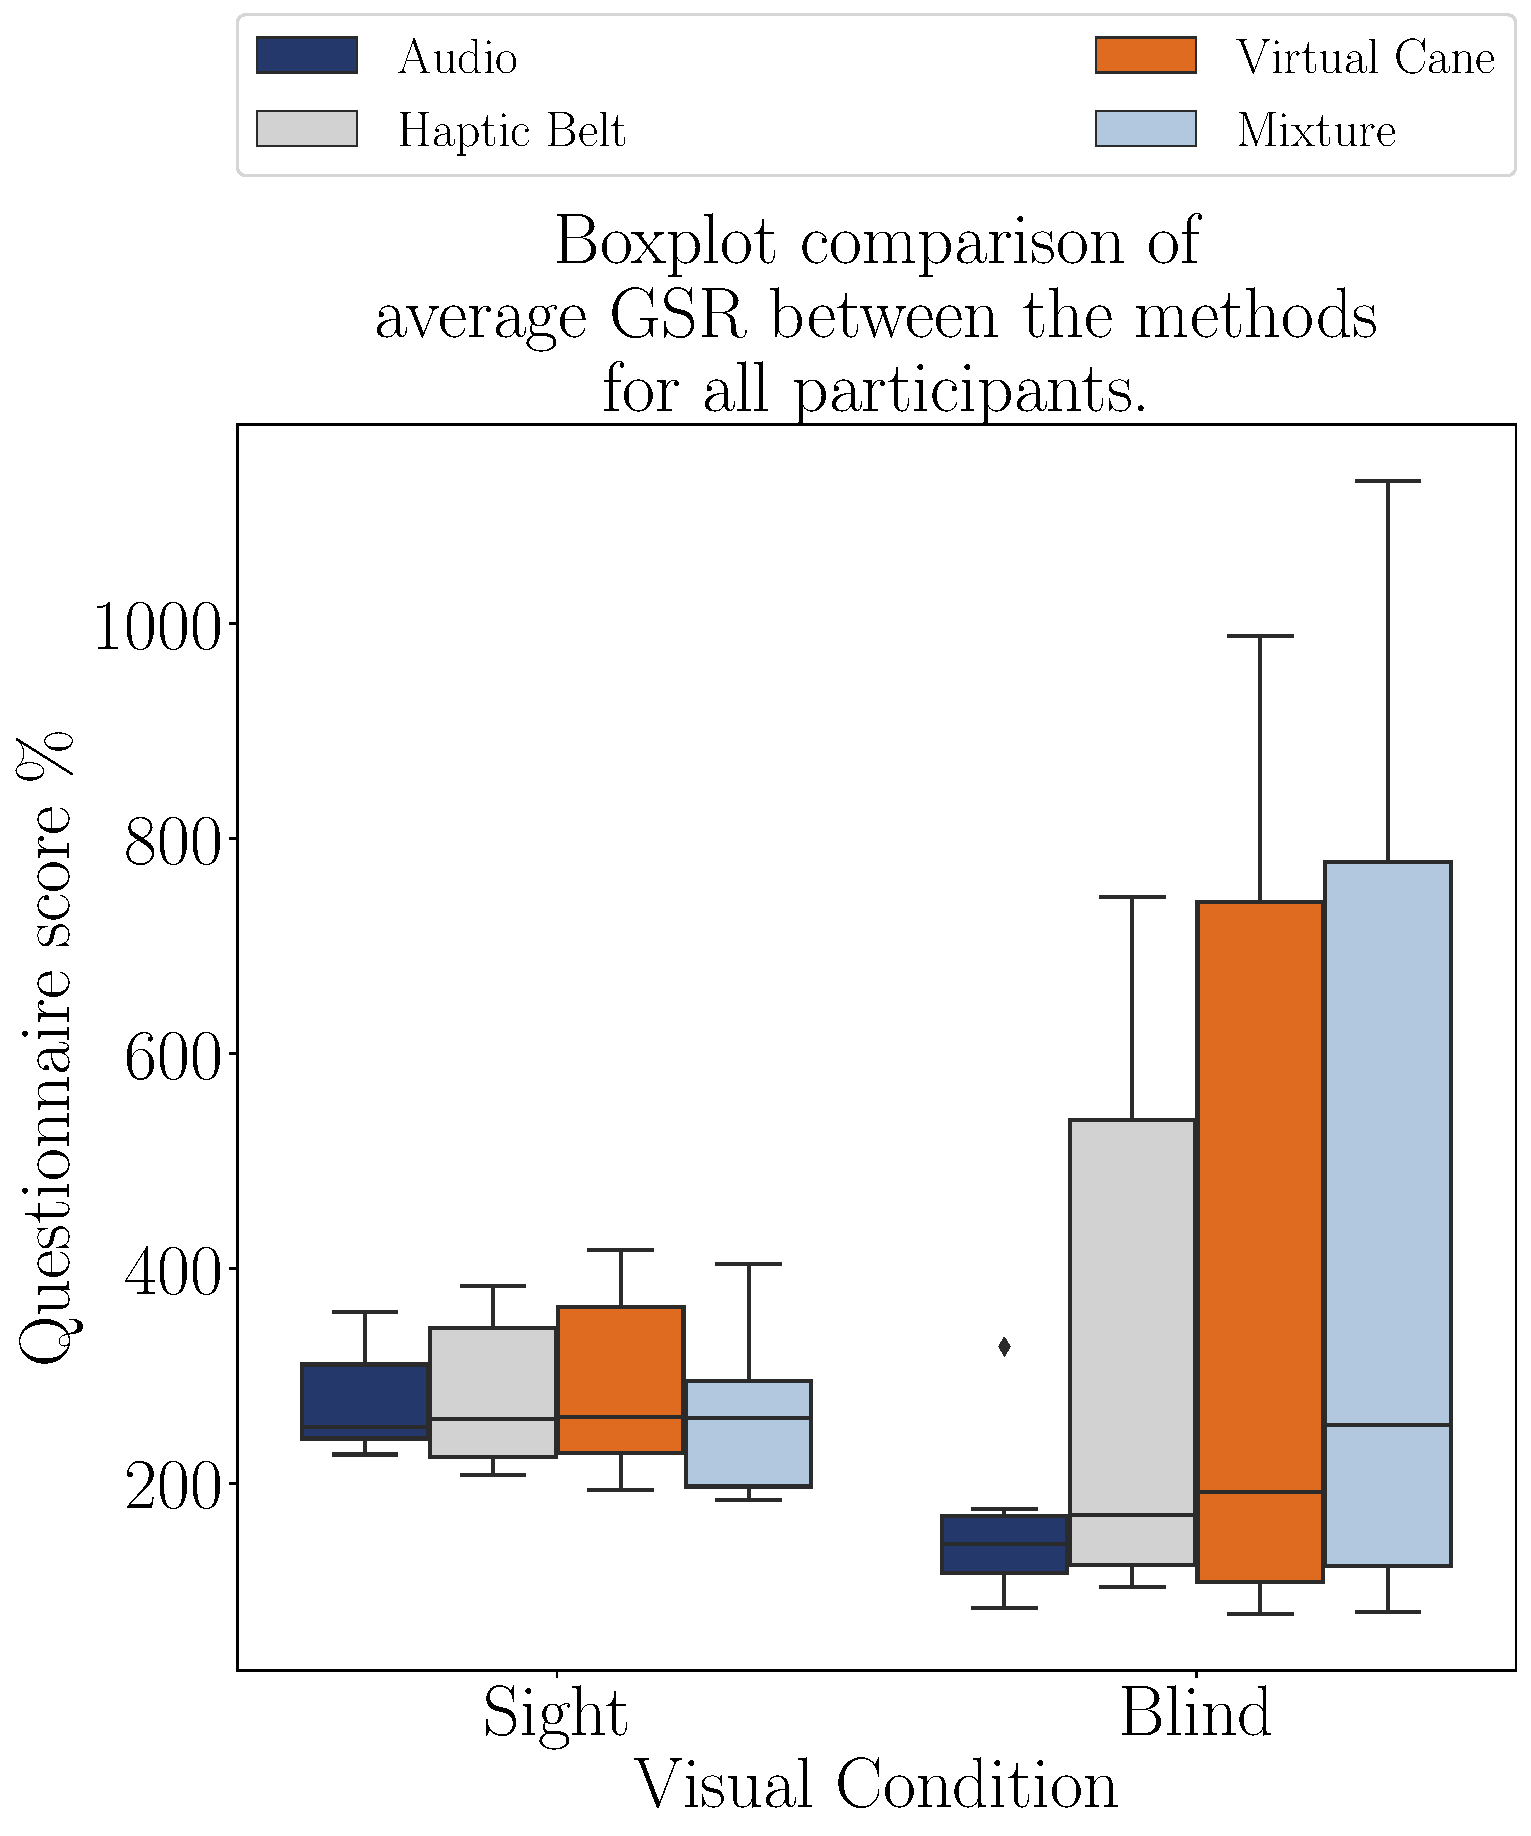
\includegraphics[width = \textwidth]{Resultados/GSR/Figuras/pdf/boxplot_gsr_avg_4_scene.pdf}
        \caption{Boxplot of the average GSR of the participants grouped by method.}
        \label{fig:boxplot_gsr_avg_4_scene}
    \end{minipage}
    \begin{minipage}{0.075\textwidth}
        \hfill
    \end{minipage}
    \begin{minipage}{0.45\textwidth}
        \centering
        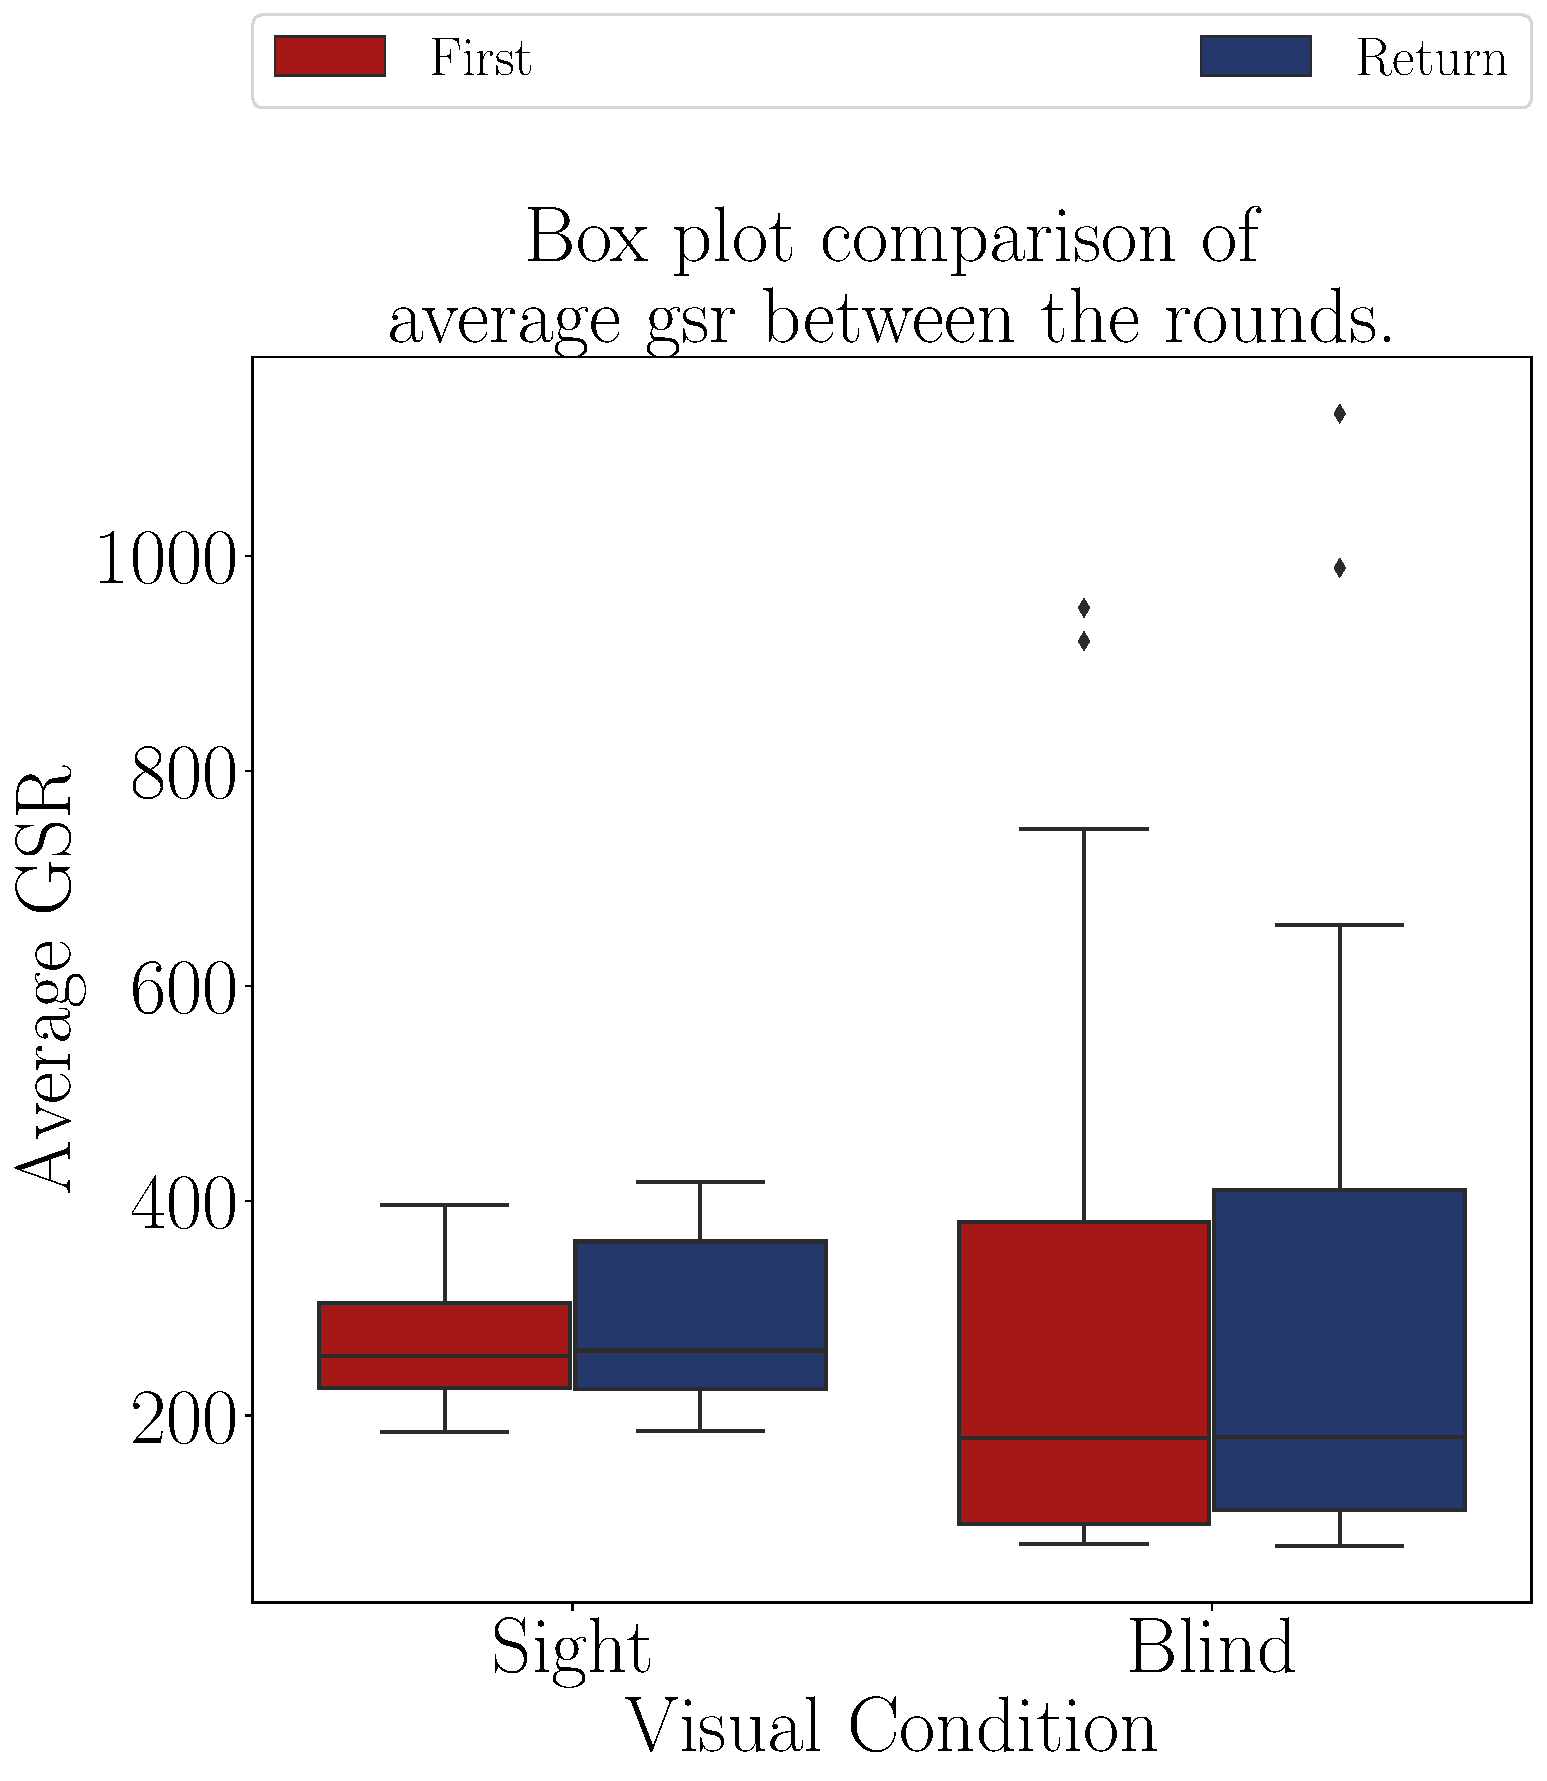
\includegraphics[width = \textwidth]{Resultados/GSR/Figuras/pdf/boxplot_gsr_avg_4_rounds.pdf}
        \caption{Boxplot of the average GSR of the participants grouped by round.}
        \label{fig:boxplot_gsr_avg_4_rounds}
    \end{minipage}
\end{figure}

Figures \ref{fig:qqplot_gsr_two_way_sight} and \ref{fig:residplot_gsr_two_way_sight} bring the QQ Plot and residual distribution. The results from ANOVA are presented in Table \ref{tab:blocanova_gsr_two_way_blind_sight}. In the case of blind participants, the p-value for the method is just slightly over the threshold, indicating a possible influence of the method. The same does not happen with sighted participants, where the p-value of the method factor is the highest and well above the 0.05 threshold.
 
%The Table \ref{tab:gsr_average_group_noBase} shows the average skin conductance variation of both samples. It also shows that the presence of a haptic device increases the GSR, whilst the sight user had a basically constant GSR.
%
%
\begin{table}[!htb]
\centering
\caption{Average GSR variation grouped by participant and visual condition}
\label{tab:gsr_average_group_noBase}
\begin{tabular}{lrrrrr}
\toprule
{} &     Audio & \begin{tabular}[c]{@{}l@{}}Haptic\\ Belt\end{tabular} & \begin{tabular}[c]{@{}l@{}}Virtual\\ Cane\end{tabular} &   Mixture \\
Visual Condition &           &                                                       &                                                        &           \\
\midrule
Blind            &  164.10\% &                                              327.01\% &                                               409.57\% &  459.15\% \\
Sight            &  276.80\% &                                              282.80\% &                                               291.73\% &  265.50\% \\
\bottomrule
\end{tabular}
\end{table}



\begin{table}[!htb]
    \caption{Anova p-value for the skin conductance average on each method}
    \label{tab:blocanova_gsr_two_way_blind_sight}
\begin{minipage}{0.45\textwidth}
    \subcaption{Blind participants}
    \input{Resultados/GSR/Tabelas/blocanova_gsr_two_way_blindsemBegin.tex}
\end{minipage}
\begin{minipage}{0.45\textwidth}
    \subcaption{Sight participants}
    \input{Resultados/GSR/Tabelas/blocanova_gsr_two_way_sightsemBegin.tex}
\end{minipage}
\end{table}

\begin{figure}[!htb]
    \centering
    %\vspace{-15.0cm}
    \begin{minipage}{0.45\textwidth}
        \centering
        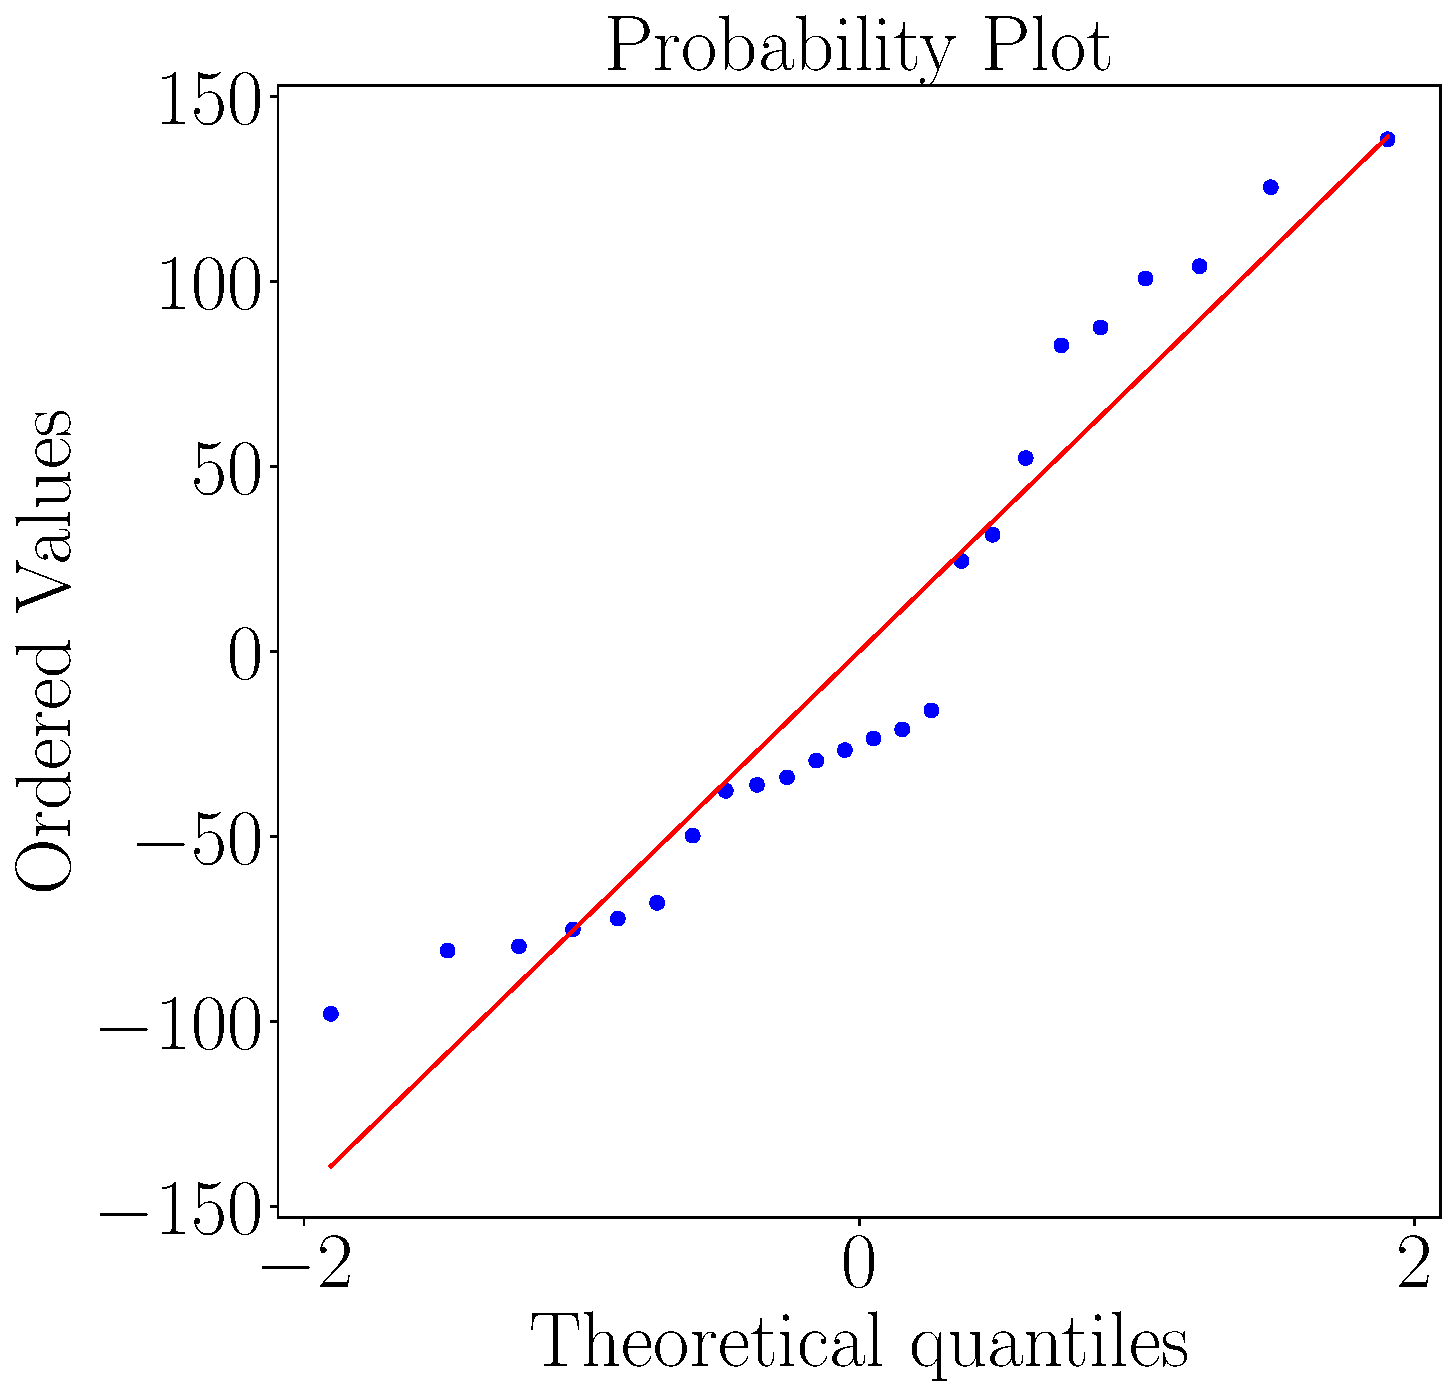
\includegraphics[width = \textwidth]{Resultados/GSR/Figuras/pdf/qqplot_gsr_two_way_sight.pdf}
        \caption{QQ plot of the average skin conductance of the sight participants on each method.}
        \label{fig:qqplot_gsr_two_way_sight}
    \end{minipage}
    \begin{minipage}{0.075\textwidth}
        \hfill
    \end{minipage}
    \begin{minipage}{0.45\textwidth}
        \centering
        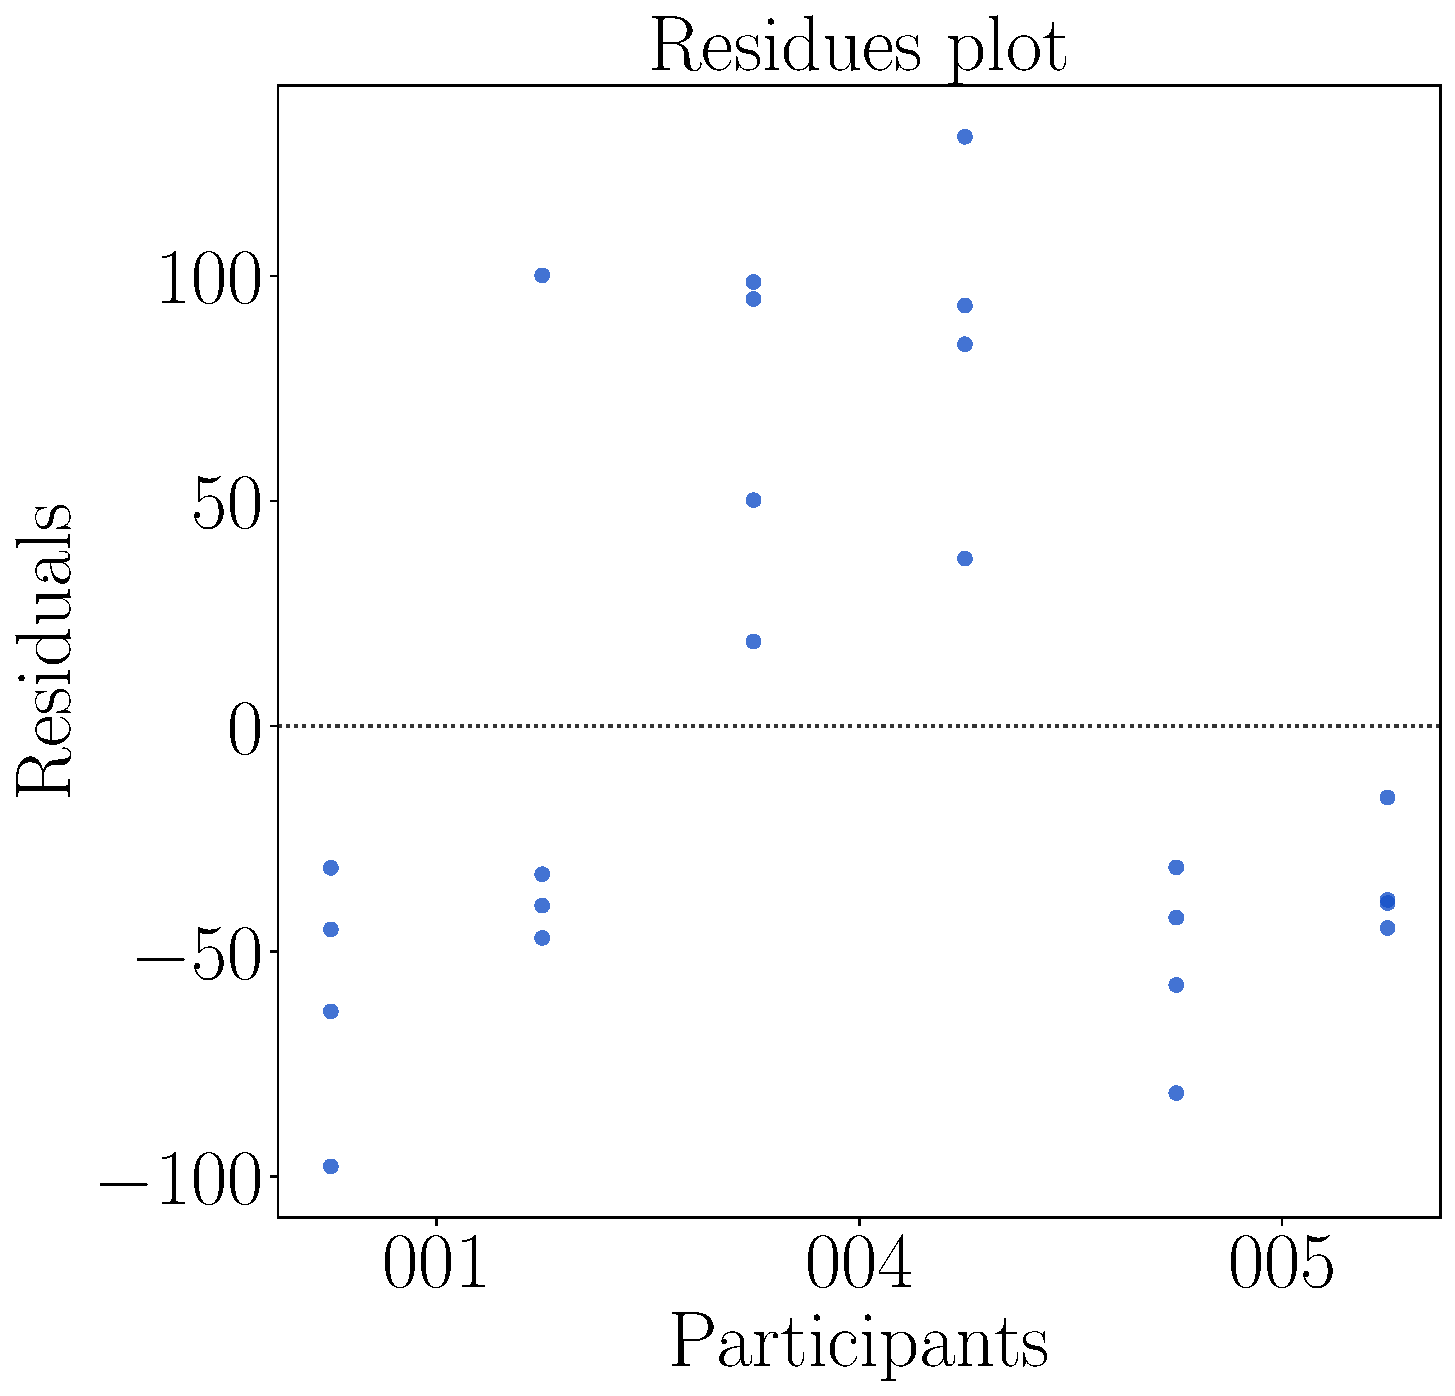
\includegraphics[width = \textwidth]{Resultados/GSR/Figuras/pdf/residplot_gsr_two_way_sight.pdf}
        \caption{Residual plot of the average skin conductance score the sight participants on each method.}
        \label{fig:residplot_gsr_two_way_sight}
    \end{minipage}
\end{figure}

\FloatBarrier